%============================================================================
% tento soubor pouzijte jako zaklad
% (c) 2008 Michal Bidlo
% E-mail: bidlom AT fit vutbr cz
%============================================================================
% kodovaní: iso-8859-2 (zmena prikazem iconv, recode nebo cstocs)
%----------------------------------------------------------------------------
% zpracování: make, make pdf, make desky, make clean
% připomínky posílejte na e-mail: bidlom AT fit.vutbr.cz
% vim: set syntax=tex encoding=latin2:
%============================================================================
\documentclass[cover]{fitthesis} % odevzdani do wisu - odkazy, na ktere se da klikat
%\documentclass[cover,print]{fitthesis} % pro tisk - na odkazy se neda klikat
%\documentclass[english,print]{fitthesis} % pro tisk - na odkazy se neda klikat
%      \documentclass[english]{fitthesis}
% * Je-li prace psana v anglickem jazyce, je zapotrebi u tridy pouzit 
%   parametr english nasledovne:
%      \documentclass[english]{fitthesis}
% * Neprejete-li si vysazet na prvni strane dokumentu desky, zruste 
%   parametr cover

% zde zvolime kodovani, ve kterem je napsan text prace
% "latin2" pro iso8859-2 nebo "cp1250" pro windows-1250, "utf8" pro "utf-8"
%\usepackage{ucs}
\usepackage[utf8]{inputenc}
\usepackage[T1, IL2]{fontenc}
\usepackage{url}
\DeclareUrlCommand\url{\def\UrlLeft{<}\def\UrlRight{>} \urlstyle{tt}}

%zde muzeme vlozit vlastni balicky
\usepackage{listings}

% =======================================================================
% balíček "hyperref" vytváří klikací odkazy v pdf, pokud tedy použijeme pdflatex
% problém je, že balíček hyperref musí být uveden jako poslední, takže nemůže
% být v šabloně
\ifWis
\ifx\pdfoutput\undefined % nejedeme pod pdflatexem
\else
  \usepackage{color}
  \usepackage[unicode,colorlinks,hyperindex,plainpages=false,pdftex]{hyperref}
  \definecolor{links}{rgb}{0.4,0.5,0}
  \definecolor{anchors}{rgb}{1,0,0}
  \def\AnchorColor{anchors}
  \def\LinkColor{links}
  \def\pdfBorderAttrs{/Border [0 0 0] }  % bez okrajů kolem odkazů
  \pdfcompresslevel=9
\fi
\fi

%Informace o praci/projektu
%---------------------------------------------------------------------------
\projectinfo{
  %Prace
  project=BP,            %typ prace BP/SP/DP/DR
  year=2016,             %rok
  date=\today,           %datum odevzdani
  %Nazev prace
  title.cs={Webová platforma pro tvorbu her},  %nazev prace v cestine
  title.en={Web Platform for Game Development}, %nazev prace v anglictine
  %Autor
  author={Filip Gulán},   %jmeno prijmeni autora
  %author.title.p=Bc., %titul pred jmenem (nepovinne)
  %author.title.a=PhD, %titul za jmenem (nepovinne)
  %Ustav
  department=UIFS, % doplnte prislusnou zkratku: UPSY/UIFS/UITS/UPGM
  %Skolitel
  supervisor= Radek Burget, %jmeno prijmeni skolitele
  supervisor.title.p=Ing.,   %titul pred jmenem (nepovinne)
  supervisor.title.a={Ph.D.},    %titul za jmenem (nepovinne)
  %Klicova slova, abstrakty, prohlaseni a podekovani je mozne definovat 
  %bud pomoci nasledujicich parametru nebo pomoci vyhrazenych maker (viz dale)
  %===========================================================================
  %Klicova slova
  keywords.cs={webova platforma, API, HTML5 hra, Nette, Bootstrap, Phaser}, %klicova slova v ceskem jazyce
  keywords.en={web platform, API, HTML5 game, Nette, Bootstrap, Phaser}, %klicova slova v anglickem jazyce
  %Abstract
  abstract.cs={Cílem této práce je návrh a realizace moderní webové platformy pro tvorbu her. Webová platforma je určená, jak pro vývojáře HTML5/Javascript her, tak i pro hráče těchto her. Součástí práce je také webový portál a API, které zpřístupňuje služby webového portálu vývojářům her. Táto platforma je na serverové straně postavená na skriptovacím jazyku PHP za použití rámce Nette. Na klientské straně je využito HTML, CSS, Javascript a pro účely responzivniho dizajnu je využíván frontendový rámec Bootstrap. Hra, která demonstruje API je napsaná v jazyku Javascript s využitím rámce Phaser. }, % abstrakt v ceskem jazyce
  abstract.en={\colorbox{red}{TODO}}, % abstrakt v anglickem jazyce
  %Prohlaseni
  declaration={Prohlašuji, že jsem tuto bakalářskou práci vypracoval samostatně pod vedením pana Ing. Radka Burgeta, Ph.D. Uvedl jsem všechny literární prameny a publikace, ze kterých jsem čerpal.},
  %Podekovani (nepovinne)
  acknowledgment={\colorbox{red}{TODO}} % nepovinne
}

%Abstrakt (cesky, anglicky)
%\abstract[cs]{Do tohoto odstavce bude zapsán výtah (abstrakt) práce v českém jazyce.}
%\abstract[en]{Do tohoto odstavce bude zapsán výtah (abstrakt) práce v anglickém jazyce.}

%Klicova slova (cesky, anglicky)
%\keywords[cs]{Sem budou zapsána jednotlivá klíčová slova v českém jazyce, oddělená čárkami.}
%\keywords[en]{Sem budou zapsána jednotlivá klíčová slova v anglickém jazyce, oddělená čárkami.}

%Prohlaseni
%\declaration{Prohlašuji, že jsem tuto bakalářskou práci vypracoval samostatně pod vedením pana X...
%Další informace mi poskytli...
%Uvedl jsem všechny literární prameny a publikace, ze kterých jsem čerpal.}

%Podekovani (nepovinne)
%\acknowledgment{V této sekci je možno uvést poděkování vedoucímu práce a těm, kteří poskytli odbornou pomoc
%(externí zadavatel, konzultant, apod.).}

\begin{document}
  % Vysazeni titulnich stran
  % ----------------------------------------------
  \maketitle
  % Obsah
  % ----------------------------------------------
  \tableofcontents
  
  % Seznam obrazku a tabulek (pokud prace obsahuje velke mnozstvi obrazku, tak se to hodi)
  % \listoffigures
  % \listoftables 

  % Text prace
  % ----------------------------------------------
  
  \definecolor{lightgray}{rgb}{.9,.9,.9}
\definecolor{darkgray}{rgb}{.4,.4,.4}
\definecolor{purple}{rgb}{0.65, 0.12, 0.82}
\lstdefinelanguage{JavaScript}{keywords={break, case, catch, continue, debugger, default, delete, do, else, false, finally, for, function, if, in, instanceof, new, null, return, switch, this, throw, true, try, typeof, var, void, while, with},morecomment=[l]{//},morecomment=[s]{/*}{*/},morestring=[b]',morestring=[b]",ndkeywords={class, export, boolean, throw, implements, import, this},keywordstyle=\color{blue}\bfseries,ndkeywordstyle=\color{darkgray}\bfseries,identifierstyle=\color{black},commentstyle=\color{purple}\ttfamily,stringstyle=\color{red}\ttfamily,sensitive=true}
\lstset{language=JavaScript,backgroundcolor=\color{lightgray},extendedchars=true,basicstyle=\footnotesize\ttfamily,showstringspaces=false,showspaces=false,numbers=left,numberstyle=\footnotesize,numbersep=9pt,tabsize=2,breaklines=true,showtabs=false,captionpos=b}
\renewcommand{\lstlistingname}{Kód}
  
  %=========================================================================
% (c) Filip Gulán, 2016

\chapter{Úvod}
\label{chap:uvod}
V minulosti v oblasti herného priemyslu existovalo niekoľko webových platforiem, ktoré sprostredkovali rôzne služby pre vývojárov hier. Za zmienku stoja napríklad tabuľky najlepších hráčov, správa odmien, pokročilé štatistiky prístupov, vzdialené úložisko dát a iné. Tieto služby boli orientované iba na webové hry, vytvorené technológiou Flash. Keďže samotná technológia Flash pomaly upadá, tak aj tieto služby pomaly zanikajú, alebo už zanikli. Takýmto príkladom môže byť líder sveta Flashových hier menom Mochimedia. Mobilné platformy ako Android a iOS, alebo platforma Steam začali sami oficiálne podporovať tieto služby už pri svojom vzniku. S rozmachom moderných webových technológií a ich následným rozšírením na chytré mobilné zariadenia vznikla možnosť tvorby webových hier, ktoré by fungovali v každom modernom webovom prehliadači, zahrňujúc nielen prehliadače v desktopových systémoch, ale aj v mobilných a tabletových.  Príchodom týchto HTML5/Javascript hier neexistovala žiadna webová stránka ponúkajúca podobné vyššie zmienené služby pre vývojárov. 

Príchodom webového portálu Clay.io v roku 2012 sa na vývojárov Javascriptových hier dočasne usmialo šťastie. Clay.io ponúkalo rôzne služby pre herných vývojárov, bez nutnosti mať státisíce prístupov do hry, alebo mať hru špičkovej grafickej úrovni. Služby boli dostupné pre všetkých, bez rozdielu. Avšak začiatkom roka 2015 sa Clay.io začalo orientovať iným smerom a z tejto webovej služby sa stal viac portál pre hráčov ako pre vývojárov. Už viac nebolo možné integrovať API do hociktorej hry a všetky hry, ktoré chceli byť umiestnené na portáli Clay.io a využívať jeho služby boli vyberané podľa prísnych kvalitatívnych kritérií. Taktiež hry využívajúce API bolo možné hrať iba na webovej stránke Clay.io a vývojár nesmel distribuovať hru na iné webové portáli. Týmto sa Clay.io uzavrelo a zaradilo sa vedľa iných svetových distribútorov HTML5 hier, ako holandská Boostermedia a Spilgames, alebo nemecký Softgames.

Táto bakalárska práca vznikla z dôvodu neexistencie otvorenej, modernej webovej platformy pre tvorbu hier pre všetkých bez rozdielu, ktorá by svoje služby ponúkala zadarmo. Táto webová platforma je orientovaná nielen na vývojárov Javascriptových hier, ktorý prostredníctvom API majú možnosť využívať služby platformy, ale aj na hráčov týchto vytvorených hier. Hráči by mali byť schopný hrať hry na akejkoľvek platforme, či už desktopových osobných počítačoch, alebo moderných chytrých telefónoch. Z toho dôvody by mala minimálne časť webového portálu určená hráčom byť do veľkej miery responzívna.

Nasledujúca kapitola sa venuje predstaveniu technológiám, ktoré boli využité v rámci realizácie tejto práce. Po nej nasleduje kapitola, ktorá zhrňuje už existujúce konkurenčné riešenia pre iné platformy. Návrh a implementácia sú popísané v rovnako pomenovaných kapitolách. A nakoniec priebeh a následné výsledky sú z hrnuté v kapitole Testovanie.

\chapter{Použité technológie}
\label{chap:technologie}
Pri implementácií platformy bolo nutné si dobre premyslieť, čoho sa má dosiahnuť a tak špecifikovať požiadavky na technológie, ktoré sa budú využívať. Po zhrnutí požiadaviek sa zistilo, že bude potrebný programovací jazyk pre serverovú časť, programovací a značkovací jazyk pre klientskú časť, jazyk, v ktorom bude implementované API pre vývojárov, databázu a databázový jazyk a napokon jazyk, v ktorom bude implementovaná hra demonštrujúca funkcie webovej platformy.

\section{Serverová časť}
\label{sec:server}
Pod pojmom serverová časť sa myslí všetko to, čo sa vykonáva na servery. Teda v prípade tejto práce to je hlavne generovanie webovej stránky platformy a práca s dátami uloženými v databázy. Okrem týchto vecí sa používa serverová časť pri práci s API\footnote{Application programming interface}, kedy sa využíva AJAX pre dotazovanie sa na server.

Pri výbere jazyka pre serverovú časť sa ponúkalo hneď niekoľko možností. Bolo na výber medzi PHP, Python, Java, Ruby, alebo ASP . NET. Napokon bolo vybrané PHP a zavážili hlavne vlastnosti, ktoré sú spomenuté v nasledujúcej kapitole.

\subsection{PHP}
\label{sec:php}
Hypertext Preprocessor je široko používaný a univerzálny open source\footnote{otvorený kód} skriptovací jazyk, ktorý sa obzvlášť používa na vývoj webových aplikácií a je možné ho vložiť do HTML súboru. Syntax jazyka je veľmi podobná syntaxi jazyku C. Od novších verzií sa PHP stal objektovo orientovaným a je v ňom možné používať OOP\footnote{objektovo orientované programovanie} postupy. Tento jazyk beží takmer na všetkých operačných systémoch od UNIXu cez Windows až po Mac OS X.

PHP bol zvolený pre serverovú časť hlavne kvôli tomu, že to je najrozšírenejší serverový jazyk a takmer všetci poskytovatelia hostingu ponúkajú webhosting práve s PHP a teda nenastáva problém s výberom poskytovateľa. Okrem toho PHP podporuje mnohé databázy ako MySQL, Oracle a PostgreSQL. Práve kombinácia PHP s Apache serverom a MySQL databázou je jedna z najobľúbenejších. 

\subsection{Model Controler View architektúra}
\label{sec:mvc}
MVC je architektonický vzor, ktorý sa uchytil predovšetkým pri tvorbe webových aplikácií a informačných systémov. Je súčasťou populárnych webových rámcov, ako napríklad Nette, alebo Zend. Základnou myšlienkou je oddelenie logiky od výstupu. MVC pozostáva, ako už názov napovedá, z 3 typov komponentov. Z modelu, pohľadu (view) a kontroléru. Model obsahuje všetku logiku aplikácie. Môžu sa v ňom nachádzať výpočty, alebo databázové operácie. Komponent pohľad sa zase stará o zobrazovanie výstupu užívateľovi. Obsahuje minimálne množstvo logiky, ktorá je pre výpis nutná. Tretí a posledný typ je kontrolér, ktorý komunikuje s užívateľom, modelom aj pohľadom a komponenty navzájom prepája. Príklad takejto architektúry a komunikácie medzi jednotlivými komponentami je zobrazený na nasledujúcom obrázku.
\begin{figure}[h]
  \centering
  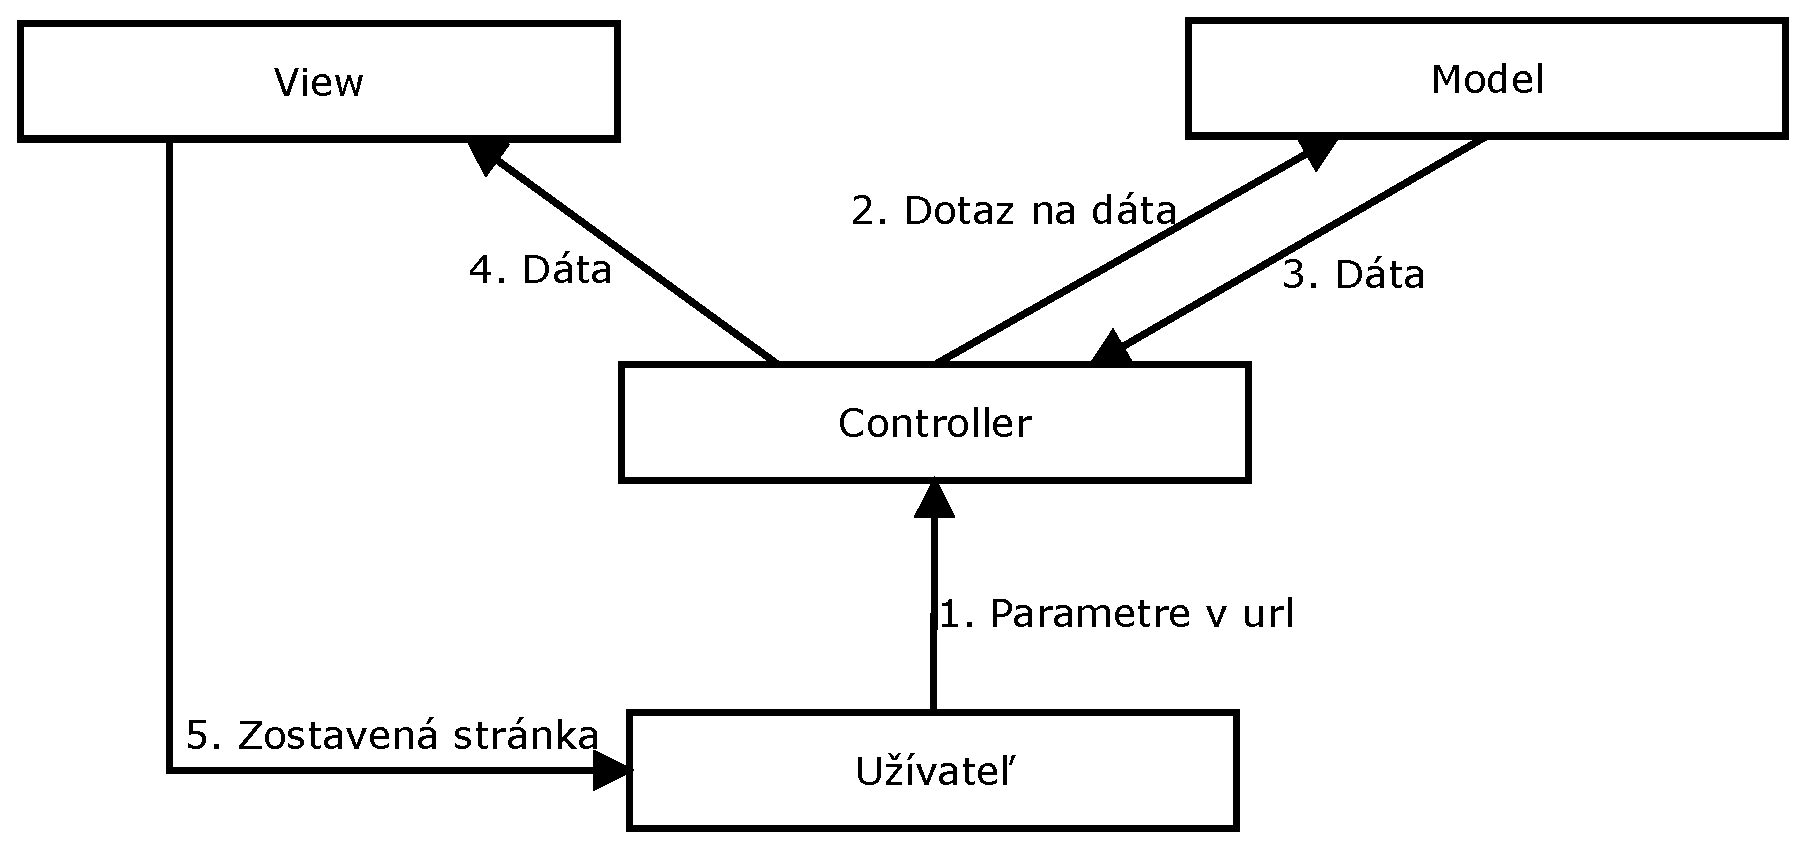
\includegraphics[scale=0.35]{fig/mvc.eps}
  \caption{Príklad MVC}
  \label{fig:mvc}
\end{figure}

\subsection{Nette}
\label{sec:nette}
PHP je síce samo o sebe mocný programovací jazyk, ale v prípade zvolenia čistého PHP, by programátor musel riešiť veľké množstvo vecí, ktoré niekto v minulosti už dávno efektívnejšie vyriešil. Okrem toho by si programátor musel dávať veľký pozor a ošetrovať početné množstvo bezpečnostných rizík. Kvôli týmto veciam bol pre účel práce vybraný aplikačný rámec Nette.

Nette je rámec napísaný v PHP5, ktorý sa zameriava na pohodlnejšie a rýchlejšie programovanie webových aplikácií a elimináciu bezpečnostných rizík. Podporuje MVC a OOP. Z veľkej časti je založený na vytváraní znovu použiteľných komponentov. K Nette patrí aj šablónovací systém Latte, ktorý zapuzdruje PHP v HTML súboroch do špeciálnych Latte makier a tým eliminuje bezpečnostné riziká. Tracy a Tester zase slúžia na hľadanie a odlaďovanie chýb. Pôvodným autorom je David Grundl, ale v súčasnosti sa o rozvoj rámcu stará Nette Foundation. Je ponúkaný pod licenciou GNU GPL a licenciou Nette (obdoba BSD licencie). Rámec sa teší veľkej obľube a taktiež početnej komunite v Čechách a na Slovensku. Minimálne požiadavky, pre správnu funkčnosť rámca, sa vyžaduje PHP verzie 5.3.1 a vyššej. Všetky požiadavky je možné overiť oficiálnym checker.php skriptom.

\section{Databázová časť}
\label{sec:databaza}
Databáza, ako prostriedok pre uloženie dát, bola zvolená hlavne kvôli vlastnosti ACID\footnote{atomickosť, konzistencia, izolovanosť a trvácnosť} a pre prístup viacerých užívateľov k databázy súčasne. Okrem iného, databázy šetria pamäťové miesto tým, že pri dobrom návrhu sa v databázy nenachádzajú redundantné dáta. Manipulácia s dátami je pomerne rýchla, pretože sa do medzi pamäte neukladá celá databáza. Nad databázou sa dajú vykonávať zložité dotazy a spájať dáta z viacerých tabuliek.  Na výber boli rôzne alternatívy ako napríklad PL/SQL, T-SQL alebo vybraný MySQL.   

\subsection{MySQL}
\label{sec:mysql}
MySQL je otvorený, viac užívateľský SQL relačný databázový server, ktorý je implementovaný vo viacerých programovacích a hlavne serverových jazykoch, napríklad v skriptovacom jazyku PHP. Je to databázový relačný systém, teda každá databáza v MySQL je tvorená z jednej alebo viacerých tabuliek, ktoré majú riadky a stĺpce. Riadky udávajú jednotlivé záznamy, stĺpce zase dátové typy jednotlivých záznamov. Práca s takouto databázou je vykonávaná pomocou takzvaných dotazov.

\section{Klientská časť}
\label{sec:klient}
Klientská časť pokrýva všetko to, čo je zobrazené užívateľovi. Teda v tomto prípade je myslená kompletná stránka, ktorej zostavovanie sa dialo z väčšej miery na servery. Aby boli informácie určené pre užívateľa zobrazené v nejakej prijateľnej a užívateľsky prívetivej podobe, tak sa vyžaduje okrem značkovacieho jazyka HTML použiť aj CSS kaskádové štýly. Keďže moderná prezentácia informácií na webových portáloch vyžaduje aj určitú ľahkosť a dynamiku, tak k tomuto účelu bol použitý celosvetovo rozšírený programovací jazyk Javascript.

\subsection{HTML}
\label{sec:html}
Hyper Text Markup Language je značkovací jazyk určený pre popis webových dokumentov, hlavne webových stránok. Najprv bol iba veľmi jednoduchá podmnožina jazyka SGML\footnote{Standard Generalized Markup Language}, ale neskôr sa z neho vyvinul samostatný štandard. HTML dokument sa popisuje pomocou HTML tagov. Každý typ HTML tagu slúži na popísanie odlišného typu obsahu dokumentu.  

V minulosti sa HTML používal na definovanie štruktúry dokumentu a aj jeho výzoru. V súčasnej dobe je HTML určené iba na zmienenú definíciu štruktúry.

\subsection{CSS}
\label{sec:css}
Kvôli tomu, že HTML sa začalo používať iba na definovanie štruktúry dokumentu a nie jeho výzoru, bol vyvinutí Cascading Style Sheets. CSS popisuje ako budú HTML tagy zobrazené na obrazovke, papieri, alebo inom médiu. CSS šetrí veľa času tým, že môže popisovať rozmiestnenie viacerých webových stránok naraz.

\subsection{Javascript}
\label{sec:javascript}
Javascript je skriptovací, prototypovo založený jazyk, ktorý sa v súčasnosti používa hlavne pri tvorbe dynamických webových prezentácií a webových stránok. Javascript beží na klientskej strane webu. Je spúšťaný väčšinou vo webových prehliadačoch. V súčasnosti Javascript podporuje väčšina webových prehliadačov a je najpoužívanejší skriptovací jazyk používaný na klientskej strane.

Bola by chyba myslieť si, že Javascript svoje uplatnenie pri tvorbe webov má iba na strane klienta. Javascript je naozaj všestranný jazyk a svoje uplatnenie nájde aj na servery napríklad v podobe Node.js. Pre účely tejto práce je avšak použitý klasický klientský Javascript spúšťaný vo webovom prehliadači.

\subsection{JQuery}
\label{sec:jquery}
JQuery je ľahká a rýchla Javascriptová knižnica, ktorá kladie dôraz na interakciu medzi Javascriptom a HTML. Syntax knižnice je navrhnutá tak, aby bolo používanie Javascriptu na stránke jendoduchšie. Medzi hlavné zjednodušenia oproti čistému Javascriptu patrí: navigácia dokumentu, výber DOM elementov, vytváranie animácií, spracovanie udalostí a veľa iných nie menej podstatných vecí. Knižnica zároveň rieši tzv. cross-browser problémy, kedy jedna věc sa môže v rôznych prehliadačoch správať odlišne.
JQuery je zároveň najobľúbenejšia a najrozšírenejšia Javascriptová knižnica, o čom svedčí nielen početná komunita, ale aj to, že je využívaná najväčšími firmami jako Google, či Microsoft.


\subsection{Bootstrap}
\label{sec:bootstrap}
Bootstrap je frontendový aplikačný rámec pre rýchle a ľahké vyvíjanie responzívnych webových stránok. Obsahuje predpripravené dizajnérske typografické šablóny založené na HTML a CSS. Hodí sa predovšetkým na prototypovanie, hlavne kvôli značnej neoriginalite vytvorených stránok, keďže väčšina stránok založená na tomto rámci vypadá veľmi podobne. Na druhú stranu, jednoduchými modifikáciami si môže skúsený dizajnér upraviť Bootstrap k svojmu obrazu.   

\subsection{Chart.js}
\label{sec:chartjs}
Chart.js je ľahká Javascriptová knižnica, pomocou ktorej je tvorba grafov z daných dát veľmi jednoduchá. Na zobrazovanie grafov používa HTML tag <canvas > do ktorého sa grafy vykresľujú. Na výber je z 6 najbežnejších typov grafov. Takto vytvorené grafy sú plne responzívne, takže môžu byť správne zobrazené, ako na stolných počítačoch s veľkou obrazovkou, tak aj na malých mobilných zariadeniach.

\section{API}
\label{sec:api}
API je v tomto prípade myslené, ako knižnica, pomocou ktorej vývojári hier pristupujú k funkciám webovej platformy. Knižnica je implementovaná v Javascripte a k funkciám platformy, ktoré sú implementované na servery sa pristupuje pomocou dotazovaním technológiou AJAX.

\subsection{AJAX}
\label{sec:ajax}
Asynchronous Javascript and XML je súhrné označenie technológie, ktorá umožňuje meniť obsah stránok bez toho, aby bolo nutné ich celé znova načítať zo servera. Hlavná výhoda spočíva v tom, že sa prenáša značne menšie množstvo dát. AJAX nieje samostatný programovací jazyk ani technológia sama o sebe, ako by sa mohlo zdať, je to skôr kombinácia niekoľkých prvkov. Je založený na internetových štandardoch, a používa kombináciu HMLHttpRequest pre získanie dát zo servera a Javascript/DOM pre zobrazenie a použitie dát. Väčšinou sa používa spolu s Javascriptom, ale nie je to podmienka, lebo je podporovaný aj v iných programovacích jazykoch.  
\begin{figure}[h]
  \centering
  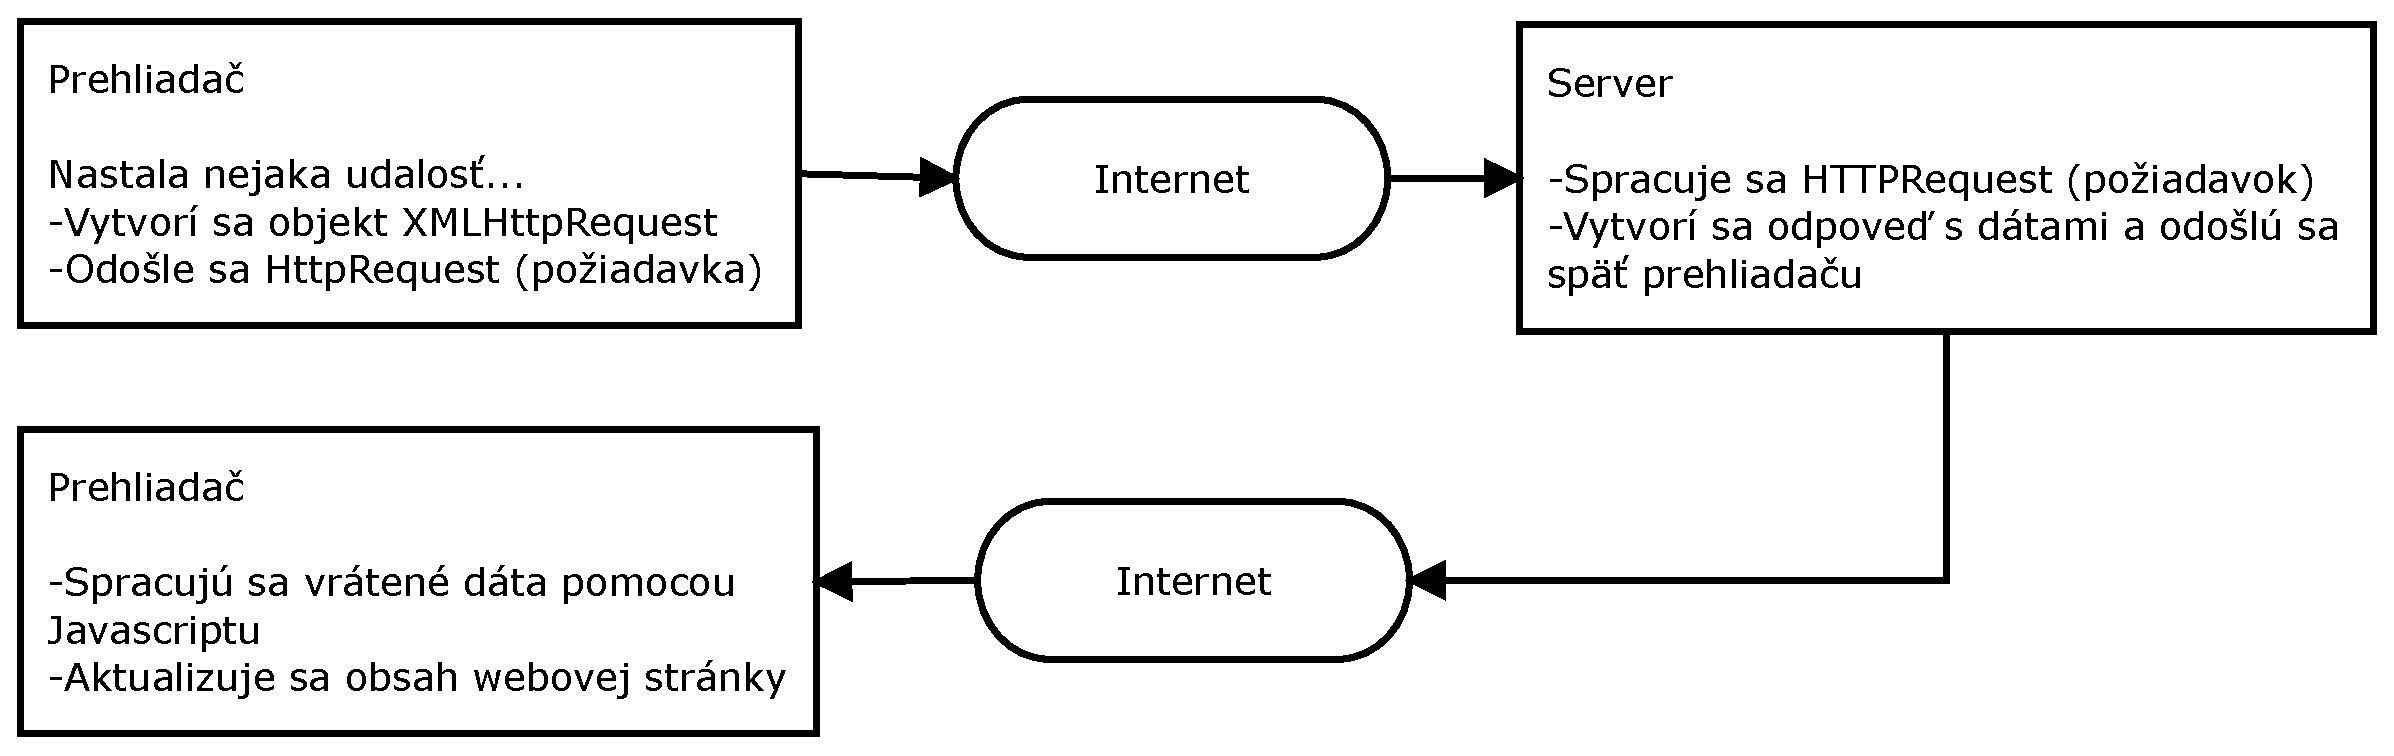
\includegraphics[scale=0.35]{fig/ajax.eps}
  \caption{Neblokujúca komunikácia so serverom pomocou AJAXu}
  \label{fig:ajax}
\end{figure}

\subsection{CORS}
\label{sec:cors}
Klasický javascript je limitovaný tzv. Same origin policy, z toho dôvodu nie je možné prijímať odpoveďe z domény, keď stránka, alebo hra, ktorá požiadavok má inú doménu. 

Tento známy, hore popísaný problém rieši Cross-origin resource sharing. CORS je vlastne mechanizmus, ktorý povoluje zakázané zdroje na webovej stránke aby boli požiadané z inej domény ako z domény z ktorej zdroje pochádzajú. Pre použitie tohto mechanizmu musí nastať zmena pri tvorbe požiadavku na klientovi, a je treba povoliť CORS na servery. Prehliadač musí posielať nastavenie Origin: doména v http hlavičke. Na servery zase musí byť nastavené povolenie Acces-Control-Allow-Origin: * (* znamená že budú povolené všetky domény).

\section{Hra}
\label{sec:hra}
Pre demonštračnú hru sa ponúkalo buďto použiť klasický Javascript, čo ale nie je príliš rozšírená forma tvorby Javascript/HTML5 hier, alebo použiť jeden z početného množstva aplikačných rámcov, ktoré sú určené špeciálne na tvorbu hier. Na výber bol Ease.js, Tree.js, Panda.js, melon.js, Kiwi.js, alebo Phaser.js a mnoho ďalších. Bol vybraný Phaser.js, pretože to je jeden z najpoužívanejších a najbežnejších Javascriptových rámcov určených pre programovanie hier, o čom svedčí hlavne početná komunita okolo tohto rámca a fakt, že aj mnohé firmy z oblasti herného biznisu, ako Boostermedia, pracujú práve s týmto rámcom. 

\subsection{Phaser}
\label{sec:phaser}
Phaser je Javascriptový aplikačný rámec určený špeciálne pre tvorbu hier, ako desktopových, tak aj mobilných. Je založený na renderovacom rámci pixi.js. Phaser je ľahko osvojiteľný, rýchly, je ponúkaný zadarmo a má otvorený kód. Podporuje canvas a zároveň aj webgl. Obsahuje veľké množstvo predpripravených funkcií. Tieto funkcie sú spracované tak, aby ich použitie bolo jednoduché. Príkladom môže byť stavaný preloader, fyzika, animácie, častice, rôzne módy prispôsobenia veľkosti obrazovky a iné.  

\chapter{Analýza existujúcich riešení}
\label{chap:analyza}
todo

\section{Herné služby}
todo

\subsection{Google Play Game Services}
todo

\subsection{Apple Game Center}
todo

\subsection{Mochimedia}
todo

\subsection{Clay.io}
todo

\subsection{Steam}
todo

\section{Znovupoužiteľné komponenty}
todo

\subsection{Odmeny}
todo

\subsection{Tabuľky najlepších hráčov}
todo

\subsection{Štatistiky}
todo

\subsection{Úložisko v cloude}
todo

\chapter{Návrh riešenia}
\label{chap:navrh}
todo

\chapter{Implementácia}
\label{chap:implementacia}
todo

\chapter{Testovanie}
\label{chap:testovanie}
todo

\chapter{Záver}
\label{chap:zaver}
todo












%=========================================================================
 % viz. obsah.tex

  % Pouzita literatura
  % ----------------------------------------------
\ifczech
  \bibliographystyle{czechiso}
\else 
  \bibliographystyle{plain}
%  \bibliographystyle{alpha}
\fi
  \begin{flushleft}
  \bibliography{literatura} % viz. literatura.bib
  \end{flushleft}
  \appendix
  
  \chapter{Obsah CD}
Adresárová štruktúra CD
\begin{itemize}
\item Zdrojové súbory
    \begin{itemize}
    \item Webový portál
    \item Javascriptové API
    \item Hra
    \item Databázový skript
    \end{itemize}
\item Grafika
\item Text
\end{itemize}
%\chapter{Manual}
%\chapter{Konfigrační soubor}
%\chapter{RelaxNG Schéma konfiguračního soboru}
\chapter{Plakat}

 % viz. prilohy.tex
\end{document}
